\documentclass[a4paper]{article}

\usepackage[utf8]{inputenc}
\usepackage{graphicx}

\title{GRACeFUL Visual Editor}
%\author{}
\date{\today}

\begin{document}

\maketitle
This document provides the usability and implementation details of the Graceful Visual Editor. The current prototype of the visual editor is a web-based application that is scalable and device independent. It supports stakeholder participation in visualizing different phases of a decision making process such as goal trees, CLDs, and SFD-like diagrams, by providing an interactive graphical interface in which the user can construct the model from building blocks available in a library (written in the GRACe DSL). 

\section{Introduction to Visual Editor}
The main elements of the visual editor are the Navigation tab, Control tab, and the Graph area as shown in Figure \ref{fig:layout}. The current prototype provides a widget-based implementation, in which each diagram is available as a separate entry in the navigation tab at the top. Based on the selected diagram in the navigation tab, its respective controls are loaded in the controls tab to the right. The graph area at the center is the canvas area, where the user can draw nodes and links. Please note that the current implementation does not differentiate between a parking lot and the main graph area canvas as proposed in D3.2. The user creates nodes and links, and constructs the model diagram in the same canvas. I.e., there is a single canvas in the graph area as opposed to two in the initial design.

\begin{figure}
\begin{center}
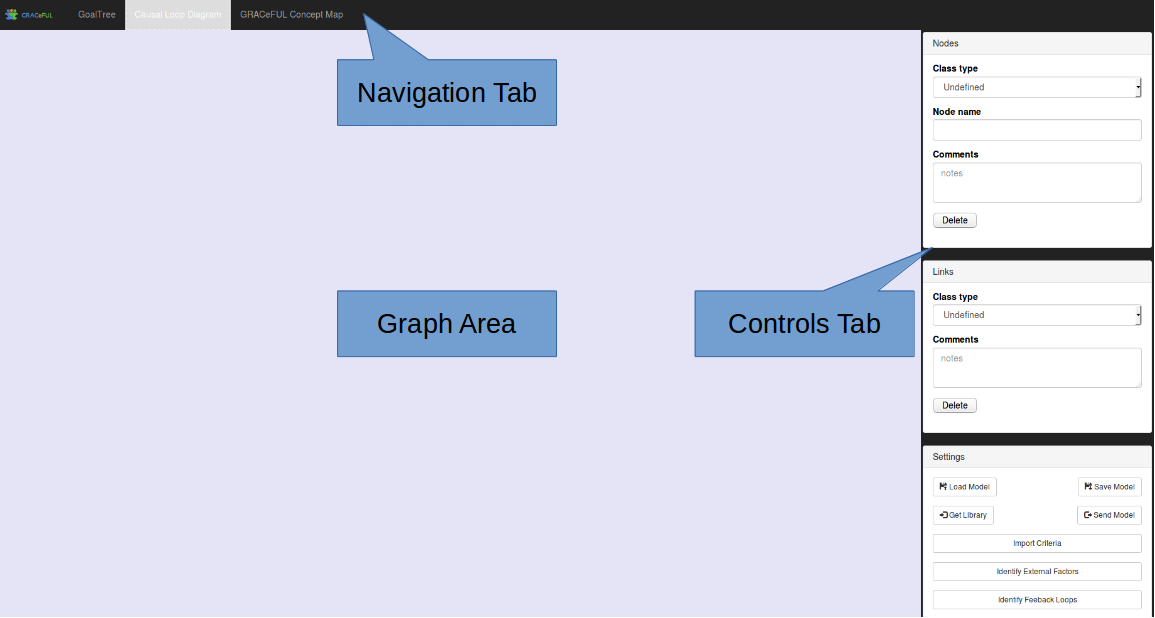
\includegraphics[height=3in,width=5in]{img/layout.png}
\caption{\small \sl Visual Editor Interface.\label{fig:layout}}
\end{center}
\end{figure}

A node can be created by double-clicking in the graph area. The label of the node is set either by double-clicking on the node or entering it in the field ‘Node name’ in the controls tab. To create a link between nodes, click the source node to get a dragger object and drag the dragger object to the target node as shown in the Figure \ref{fig:node_link}. The nodes and links can be deleted by selecting the respective node or link and click the delete button from the controls tab. Alternatively, a node or link can be deleted by hovering over it and clicking the delete icon. For every node and/or link, the editor provides the option to take notes by selecting the node and entering the content in the comments field in the control tab. The visual editor allows zooming in and out, as well as panning of the diagram. The nodes and links can also be dragged around in the graph area. 

\begin{figure}
\begin{center}
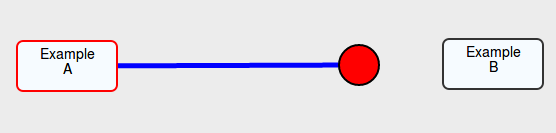
\includegraphics[height=0.75in,width=2in]{img/node_link.png}
\caption{\small \sl Create Nodes and Links.\label{fig:node_link}}
\end{center}
\end{figure}

The modeling of the GRACeFUL Concept Map (GCM) is a step-by-step process, in which the major steps are performed in separate tabs as discussed above. Currently, the goal tree, CLD, and GCM are available as separate tabs in the visual editor. 

A Goal Tree consists of a main goal as the root, which is decomposed into sub goals. The sub goals have a relation to certain criteria, which were identified by the participants. To start building a goal tree, select the goal tree tab and add nodes in the graph area with names agreed by the stakeholders. Select its respective type from the control tab to be as a main goal, sub goal or criteria, which is distinguished with different colors. Connect the nodes via links and arrange them hierarchically in the form of a tree as shown in Figure \ref{fig:goal_tree}.

\begin{figure}
\begin{center}
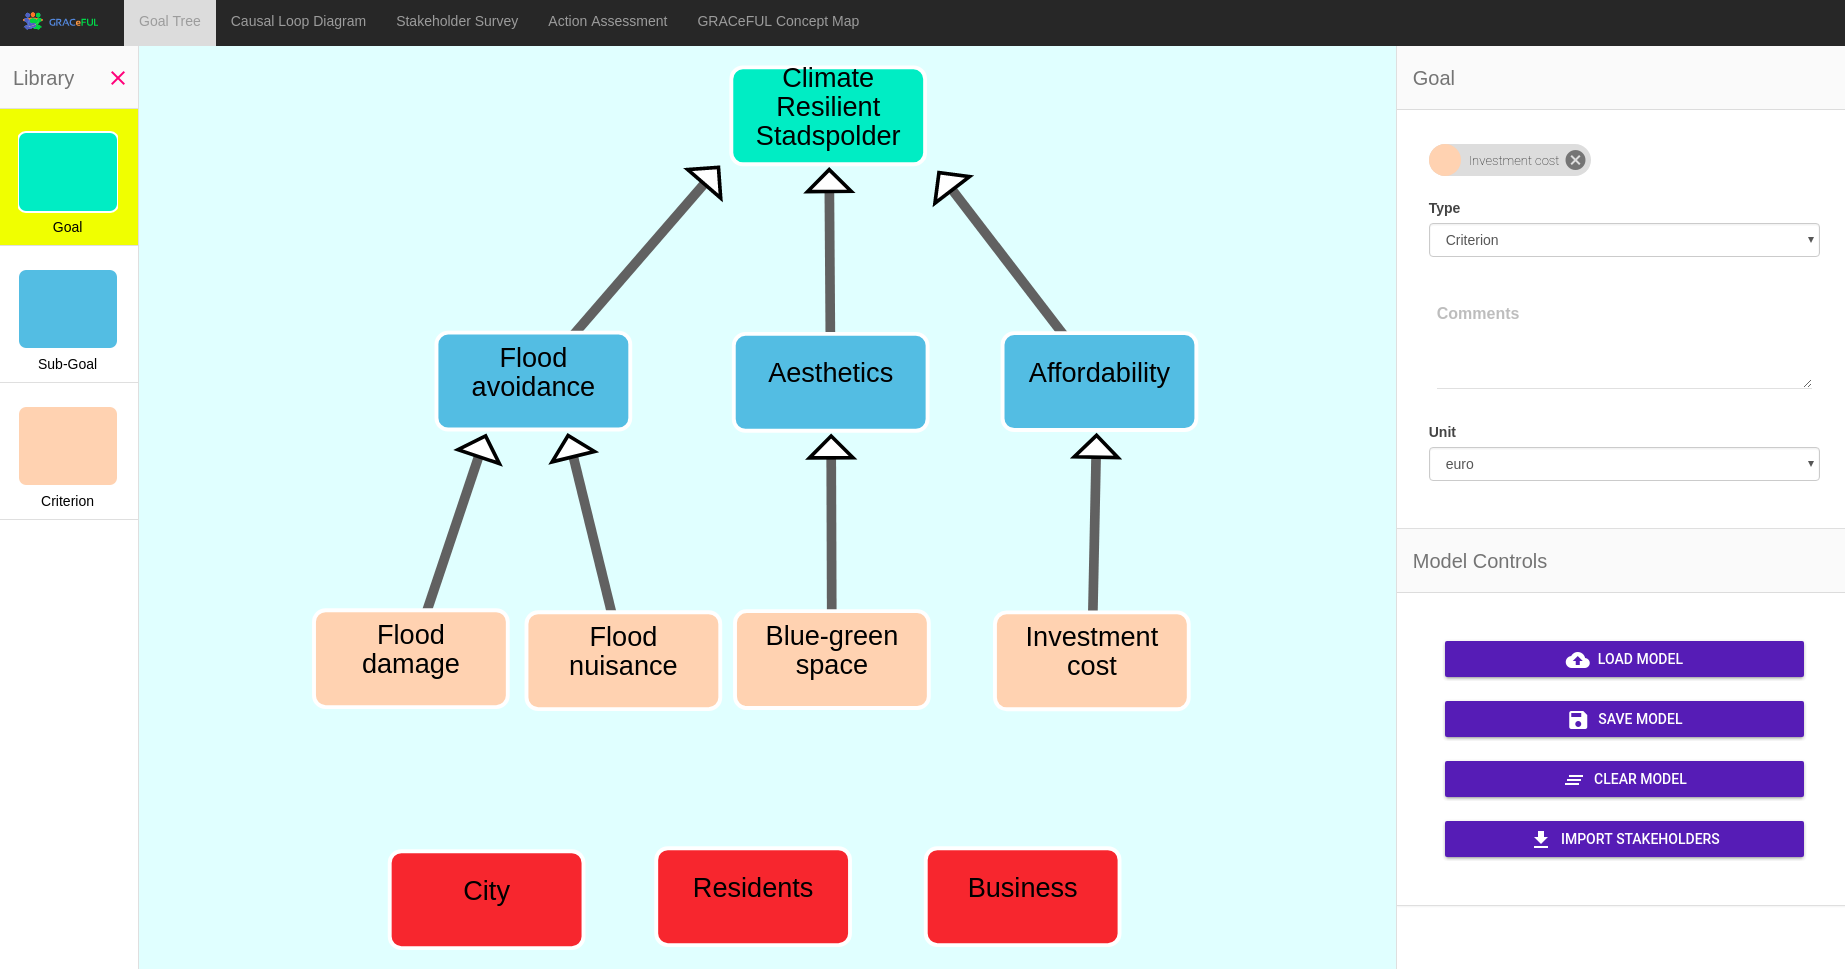
\includegraphics[height=3in,width=5in]{img/goal_tree.png}
\caption{\small \sl Goal Tree.\label{fig:goal_tree}}
\end{center}
\end{figure}

The editor allows the option to save an instance of the goal tree as a JSON file and to load a previously saved instance. Once the goal tree is built, the next step is to start modeling the GCM. GCM is represented by two distinctive graph views, namely CLD and SFD-like. 

We start modeling the GCM in the CLD view by selecting the Causal Loop Diagram tab in the editor. As a first step, the criteria that were defined in the goal tree have to be imported into the CLD editor, by clicking the button ‘Import Criteria’. Then the modeler asks the stakeholders to define the factors that influence the identified criteria. A directed link is drawn between the factors and/or criteria, to signify the relation between them as indicated by the stakeholders. For example, in the Figure \ref{fig:cld} the links with (+) sign signifies a positive causal influence, (-) signifies a negative causal relation, and (?) signifies an unknown influence. 

\begin{figure}
\begin{center}
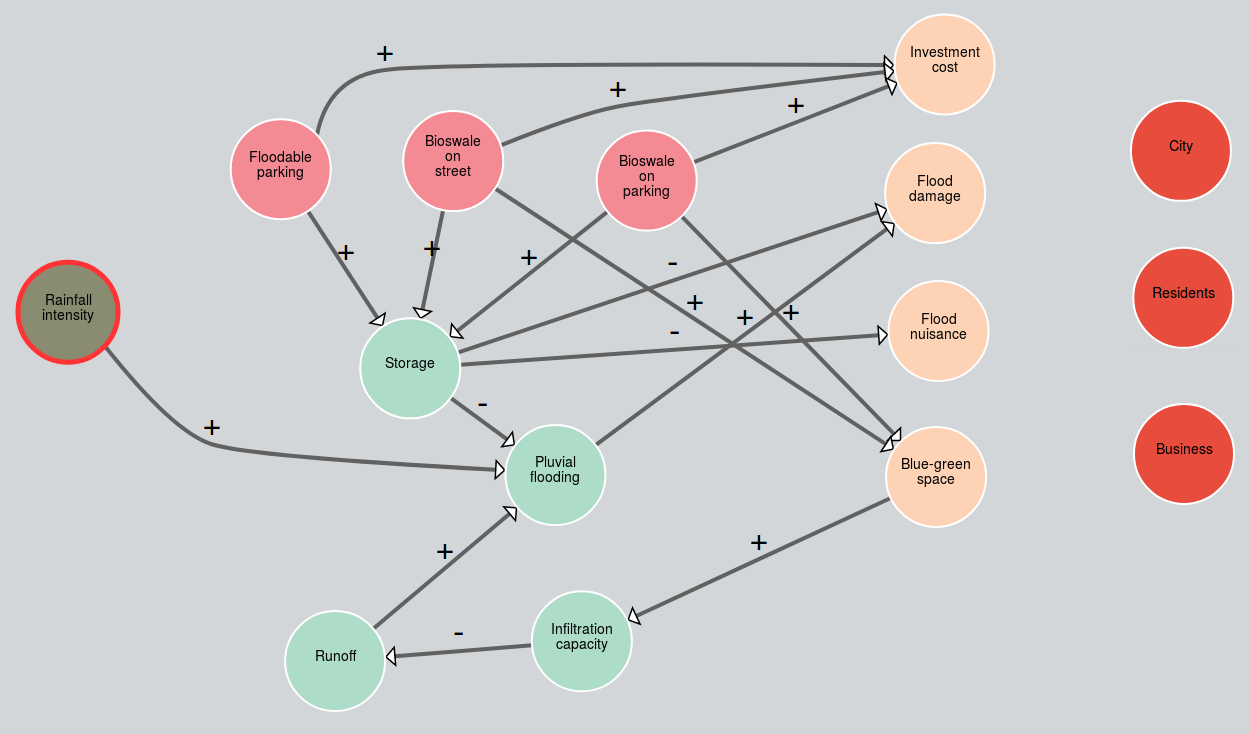
\includegraphics[height=3in,width=5in]{img/cld.png}
\caption{\small \sl Causal Loop Diagram.\label{fig:cld}}
\end{center}
\end{figure}

One important aspect in creating a CLD is that the modeler needs to match factors proposed by the participants with attributes of existing concepts in the library. The ‘Get Library’ button provides the desired functionality to fetch the library. For the communication with the library and the solver to work, the visual editor application needs to be deployed on the server. Similarly, the ‘Send Model’ sends a model to the solver for it to return feasible solutions.

The CLD editor can identify the factors that have no incoming relations. These are called external factors. The user must click the button ‘Identify External factors’ to find all the external factors in the model. For clarity, the nodes are represented by different colors to denote their type. In the Figure \ref{fig:cld}, the green nodes represent factors, the dark green node represents an external factor, and the yellow nodes represent criteria. The editor also provides a tool to find feedback loops in the model by clicking the button ‘Identify Feedback Loops’.

\begin{figure}
\begin{center}
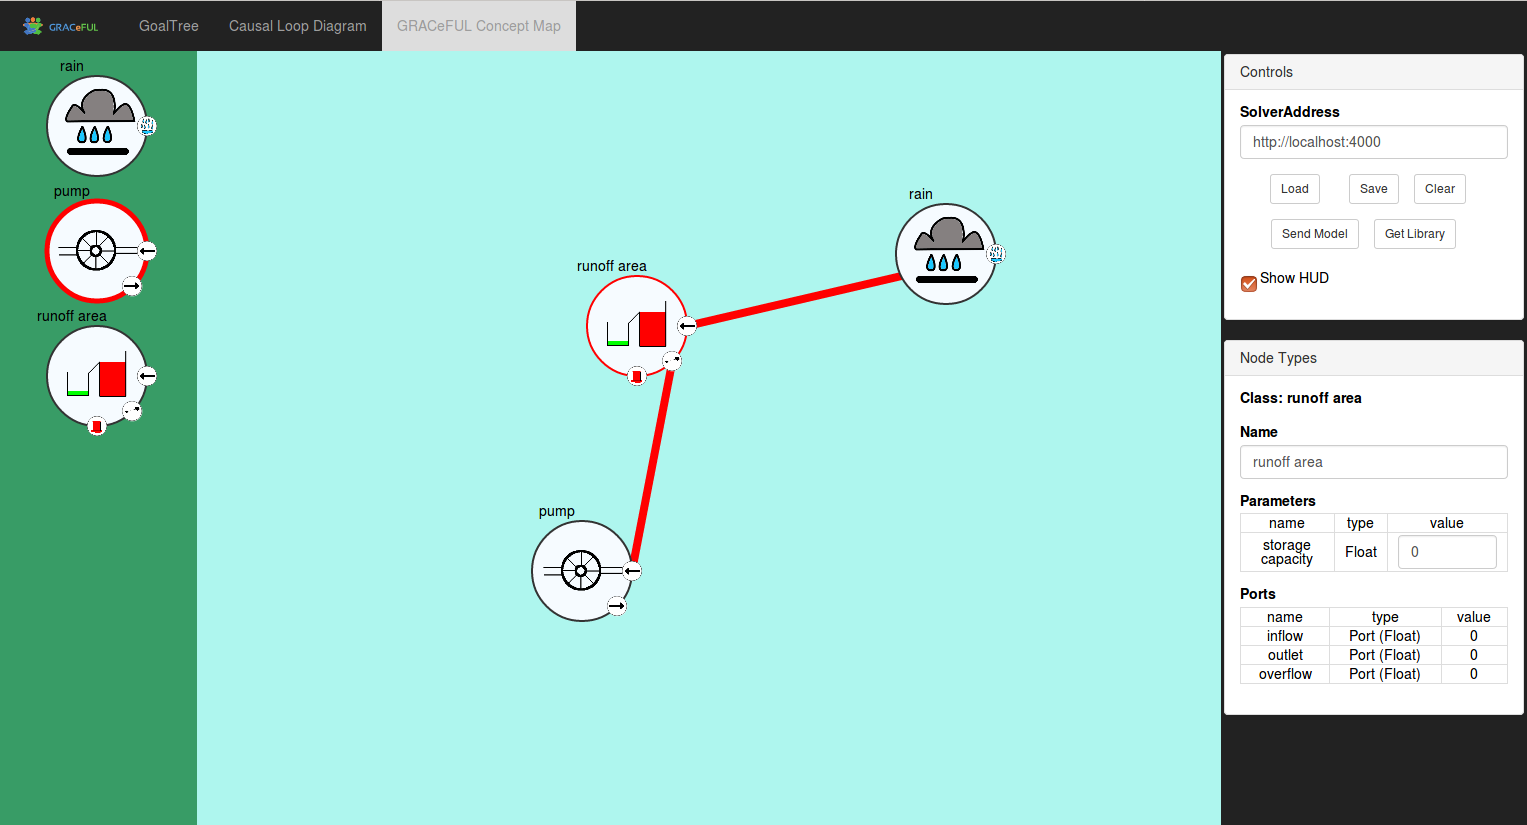
\includegraphics[height=3in,width=5in]{img/sfd_like.png}
\caption{\small \sl Graceful Concept Map.\label{fig:sfd_like}}
\end{center}
\end{figure}

The second model view is the entire GCM, including a SFD-like components and links. The latter can handle more quantitative stock-and-flow-like concepts. GCM components from the library are required to build it. On clicking the ‘Get Library’ button, the available library components are displayed on the left as shown in the Figure \ref{fig:sfd_like}. Currently, the library can be loaded on local installations, awaiting it to be deployed on the server. The SFD-like viewer from the initial prototype has been integrated into the current one. Additional features will be implemented.

Whereas in the CLD and Goal Tree editors it is clear which library concepts are being manipulated (factors, goals, causal relations), the nodes and links in the overall GCM are created by selecting them from the available library components. The control tab provides the details of the concepts such as name, parameters, and connectivity information (ports).

\section{Design and Implementation}

In this section, we provide the technical design and working of the visual editor. As introduced, it is a web-based application, which is implemented using HTML, CSS and JavaScript.  

Figure \ref{fig:visual} provides the different components of the visual editor. HTML helps in describing the structure of the application and CSS helps in better presentation of the HTML elements with proper layouts, colors, fonts, etc. JavaScript is an untyped scripting language, which helps in initializing and accessing the HTML Document Object Model (DOM) elements and also to dynamically load and change the visual appearance of the DOM. The communication module is responsible for communicating with the solver to fetch the library components and to send the model for evaluation. To have a better visual appearance, the editor uses Bootstrap, which is a HTML, CSS, and JavaScript framework. It helps in responsive design of the application, which allows it to adapt to different screen sizes, such as mobiles, tablets, desktops.

\begin{figure}
\begin{center}
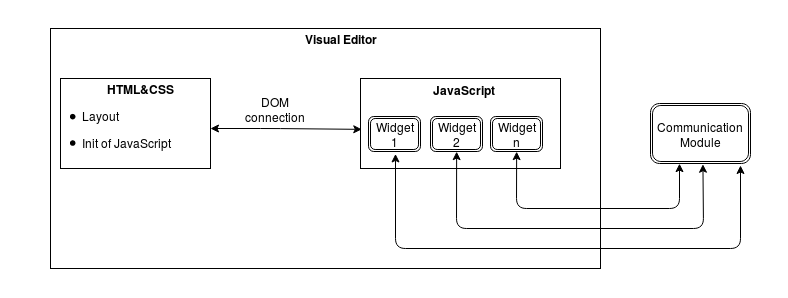
\includegraphics[height=2in,width=5in]{img/visual.png}
\caption{\small \sl Visual Editor Components.\label{fig:visual}}
\end{center}
\end{figure}

The visual editor follows a Widget-based design. The general idea is to use widgets to encapsulate different steps in the model building process. That is, the Goal Tree, CLD, SFD-like diagrams, which are available as separate tabs in the editor are individual widgets that provides its own Graph, Options/Controls, CSS styles, and type as illustrated in Figure \ref{fig:widget}.

\begin{figure}
\begin{center}
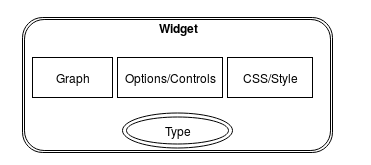
\includegraphics[height=2in,width=4in]{img/widget.png}
\caption{\small \sl Composition of a Widget.\label{fig:widget}}
\end{center}
\end{figure}

The graph is the main canvas area, which provides the rendering for nodes and links. All nodes and links are Scalable Vector Graphic (SVG) elements. We use D3.js, which is a JavaScript library for dynamic visual interaction. The options/control component contains the control buttons to edit, delete nodes and links and connect to the communication module. The CSS styles are responsible for manipulating the styles of the corresponding widget. The type signifies the widget’s type, i.e., goal tree, CLD, SFD-like diagrams, which is important for the communication module.

The widgets are rendered in the browser as separate tabs in the navigation bar that allows switching between different views of the editor. A new view can be easily created by extending the base widget and customizing it to our requirements.

\begin{figure}
\begin{center}
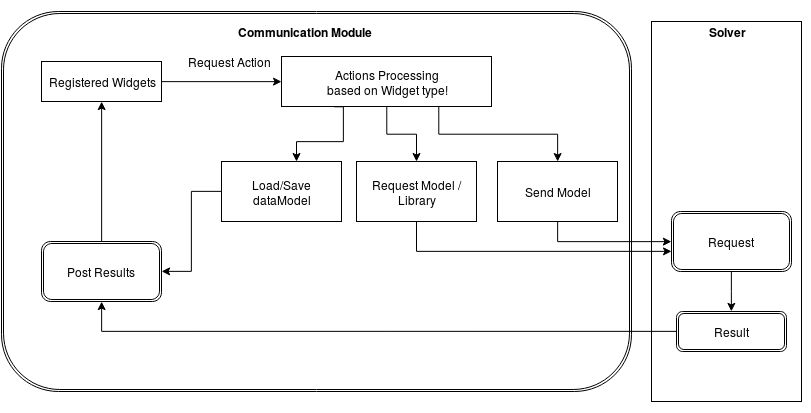
\includegraphics[height=3in,width=5in]{img/communication.png}
\caption{\small \sl Working of the Communication module.\label{fig:communication}}
\end{center}
\end{figure}

Figure \ref{fig:communication} provides the working details of the communication module. All widgets register to this module. The control component in the widget requests for action, such as load/save previous state, request library, send a model. An action is preprocessed based on the type of the widget. When sending the model, only the required data is sent to the solver. The request is either sent to the solver or, in case of loading a previous state, it directly goes to the Post results, which communicates the new results to the widget that requested this action. The widget then only needs to update itself. The communication module encapsulates the communication between the visual editor and the solver. It will be easier to maintain and modify the whole back-end communication with this module, but it requires an implementation for each widget.

Currently, the visual editor is deployed in a container to ease the process of testing while communicating to the solver. This Docker image is being deployed on a server.

\begin{figure}
\begin{center}
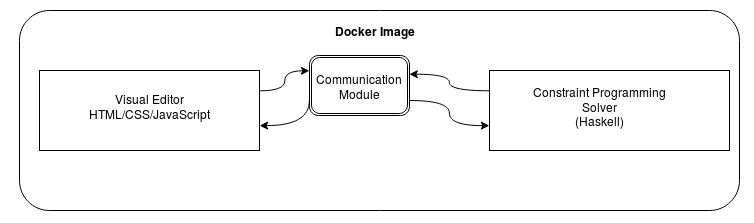
\includegraphics[height=1.5in,width=4in]{img/e2e.png}
\caption{\small \sl Docker image of the visual editor.\label{fig:e2e}}
\end{center}
\end{figure}

\end{document}